\subsection{Search Tree}
    \subsubsection{Tree terminology}
        \begin{itemize}
            \item Root: Highest node has children and no parent
            \item Order: Maximum number of child nodes (BST order = 2)
            \item Height: Maximum path length root to leaf
            \item Complete: Every level except for the lowest is filled, lowest level is filled from left to right
            \item Perfect: Every level is completely filled
            \item Full: the amount of children of every node equals either the order or 0
        \end{itemize}
    
    \subsubsection{Binary Tree Traversal}

    \subsubsection{Binary Search Tree (BST)}
        \begin{minipage}{0.49\linewidth}
            A binary search tree is a binary tree which fulfils the following:
            \begin{enumerate}
                \item Every node v stores a key
                \item Keys in the left subtree are smaller than v.key
                \item Keys in the right subtree are larger than v.key
            \end{enumerate}
        \end{minipage}
        \begin{minipage}{0.49\linewidth}
            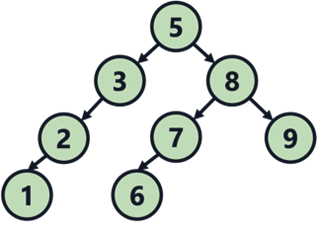
\includegraphics[width = \linewidth]{src/4_data_structure/images/bst.png}
        \end{minipage}

        {\centering\underline{\textbf{Implementation}} \par}

        {\centering\underline{\textbf{Height}} \par}

        {\centering\underline{\textbf{Search for Node}} \par}

        {\centering\underline{\textbf{Insert Node}} \par}

        {\centering\underline{\textbf{Remove Node}} \par}
        
